\documentclass{article}

\usepackage{geometry}
\geometry{letterpaper, total={7in, 10in} }
\usepackage{booktabs}
\usepackage{graphicx}
\usepackage{verbatim}

\title{CSCI 4360 Data Science II \protect\\ Project II}
\author{Ayush Kumar, Brandon Amirouche, Faisal Hossain}
\date{March 30, 2021}

\begin{document} 
	
	\maketitle
	\tableofcontents
	\newpage
	
	\section{AutoMPG}
	
	The Goal of the AutoMPG Dataset is to predict the Miles per Gallon that a car will have 
	based on a few key characteristics. 
	
	\begin{enumerate}
		\item cylinders 
		\item displacement 
		\item horsepower 
		\item weight 
		\item acceleration 
		\item model-year
	\end{enumerate}

	\subsection{Results}

	We want to find out if using feed-forward neural networks will offer some sort of advantage over 
	traditional regression modeling. The AutoMPG Dataset only has a few observations so it is highly 
	unlikely that we will be able to fully leverage the power of neural networks because our dataset 
	isn't large enough to have such complicated patterns hidden in it. In addition to this, neural networks 
	are computationally expensive and require much more hyper parameter tuning than a traditional or 
	transformed regression model. The following table summarizes the results of our findings in terms 
	of $R^2$, $\bar R^2$ $R^2_{cv}$ and $AIC$ for some traditional regression models, and some neural networks. 
	

	\begin{tabular}{|c|c|c|}
		\hline
		& $R^2$ & $\bar R^2$ \\ \hline
		Multiple Linear Regression            & 0.807 & 0.806      \\ \hline
		Quadratic Regression                  & 0.876 & 0.873      \\ \hline
		Quadratic Regression with Cross Terms & 0.883 & 0.873      \\ \hline
		Transformed Regression                & 0.851 & 0.848      \\ \hline
		Perceptron                            & 0.734 & 0.704      \\ \hline
		3 Layer Neural Network                & 0.793 & 0.790      \\ \hline
		4 Layer Neural Network                & 0.778 & 0.776      \\ \hline
	\end{tabular}

	As the directly comparable results show (some results were not stable between python and scala) we can see that the neural 
	network models offer little to no benefit in comparison to the traditional regression models. In fact 
	while the 3 and 4 layer networks perform quite well, they still lag behind a simple quadratic regression, and 
	oftentimes are not stable over repeated training loops. The 4-Layer network is especially prone to breaking, but 
	this may be because of the small size of the dataset in comparison to the number of parameters. 
	
	\subsection{Variable Selection}
	
	Forward Selection, Backward Elimination, and Stepwise Regression for the 4 models. Some turned out to be 
	not be very stable because of the randomness associated with neural networks. Nonetheless we have some results in the following graphs. 
	
	Perceptron Selection Process (Forward, Backward, Stepwise)
	
	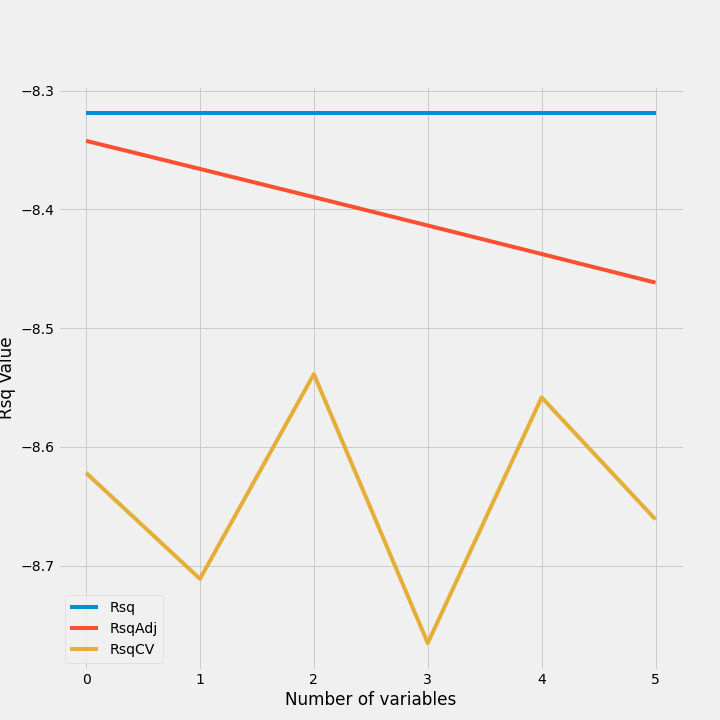
\includegraphics[scale = 0.2]{../plots/python/AutoForwardPCP.png} 
	\includegraphics[scale = 0.2]{../plots/python/BackwardPCP.png}
	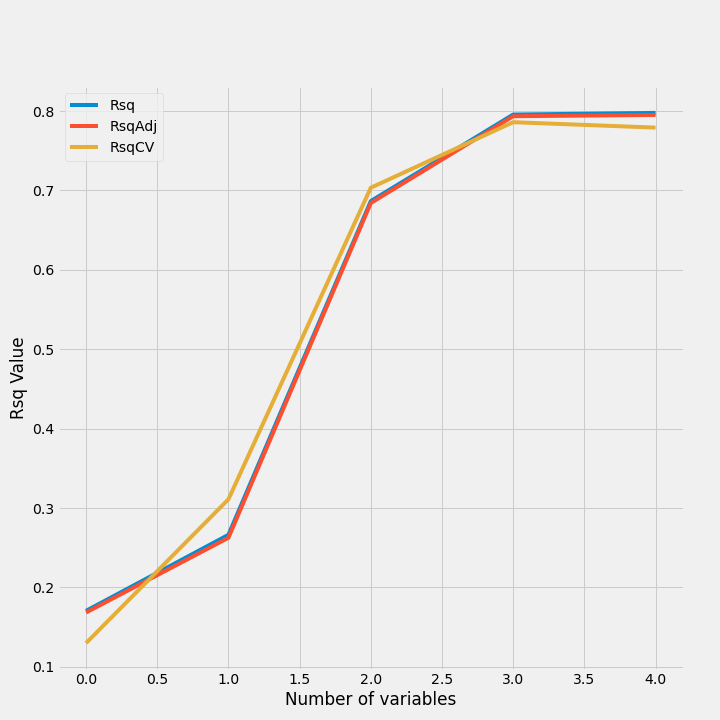
\includegraphics[scale = 0.2]{../plots/python/StepwisePCP.png}
	
	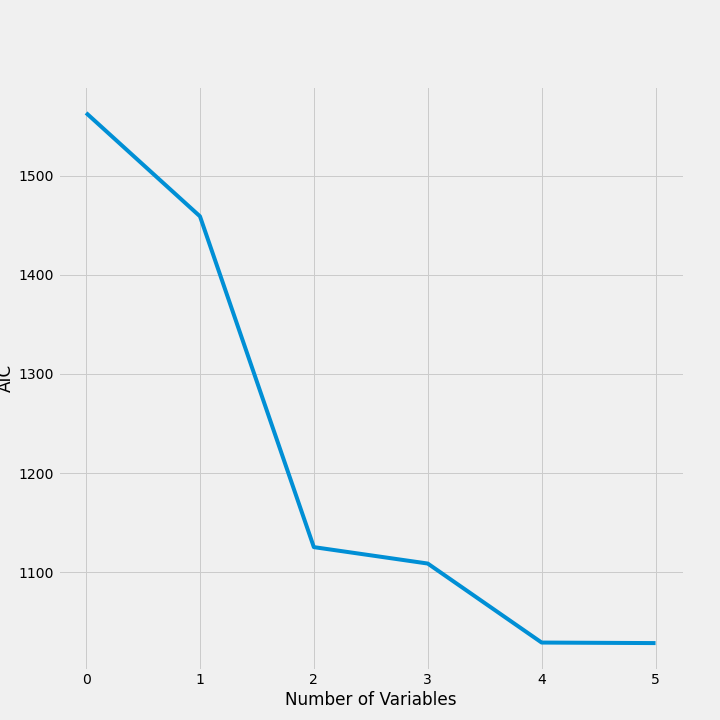
\includegraphics[scale = 0.2]{../plots/python/AICAutoForwardPCP.png} 
	\includegraphics[scale = 0.2]{../plots/python/AICBackwardPCP.png}
	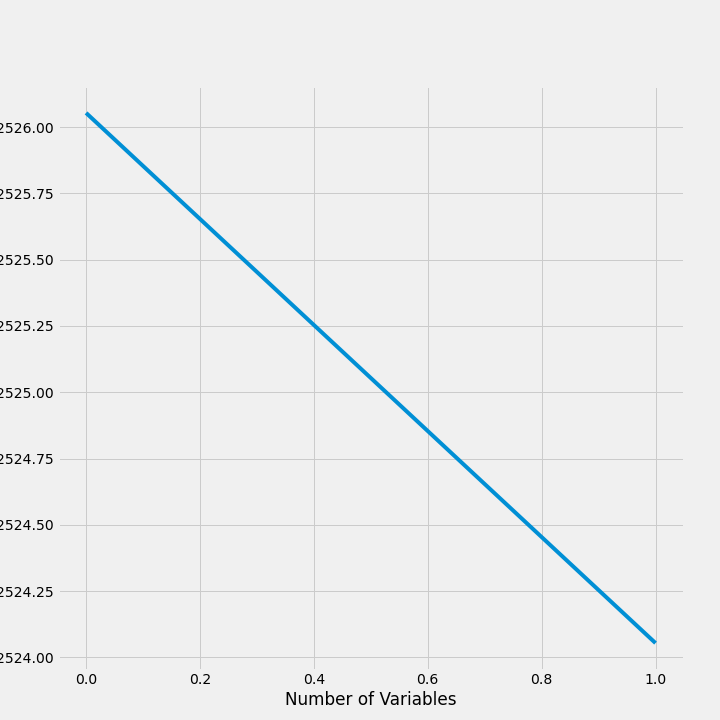
\includegraphics[scale = 0.2]{../plots/python/AICStepwisePCP.png}
	
	3 Layer Network Selection Process (Forward, Backward, Stepwise)
	
	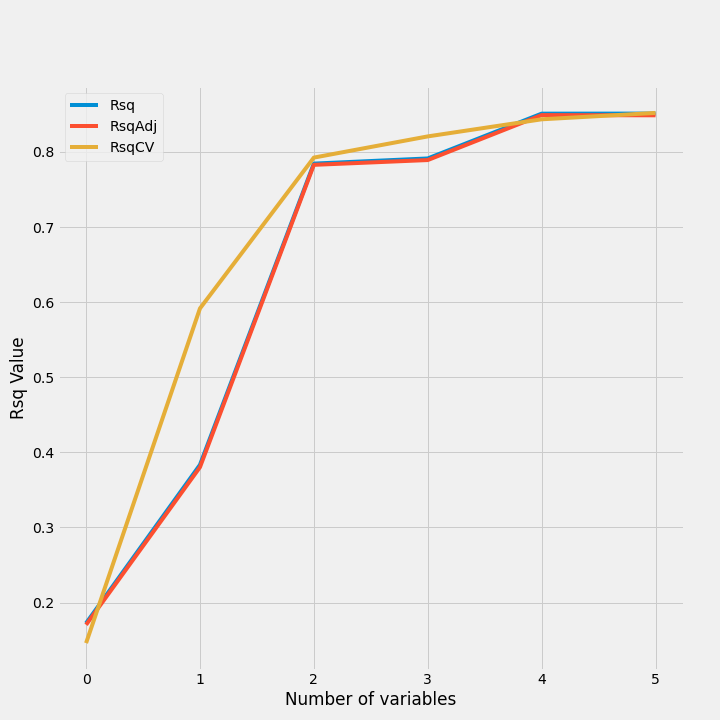
\includegraphics[scale = 0.2]{../plots/python/AutoForward3L.png} 
	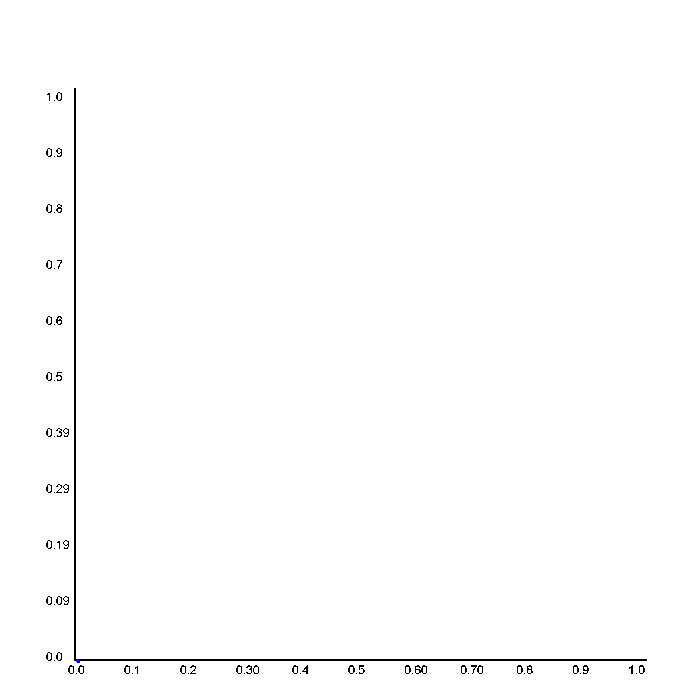
\includegraphics[scale = 0.2]{../plots/python/Backward3L.png}
	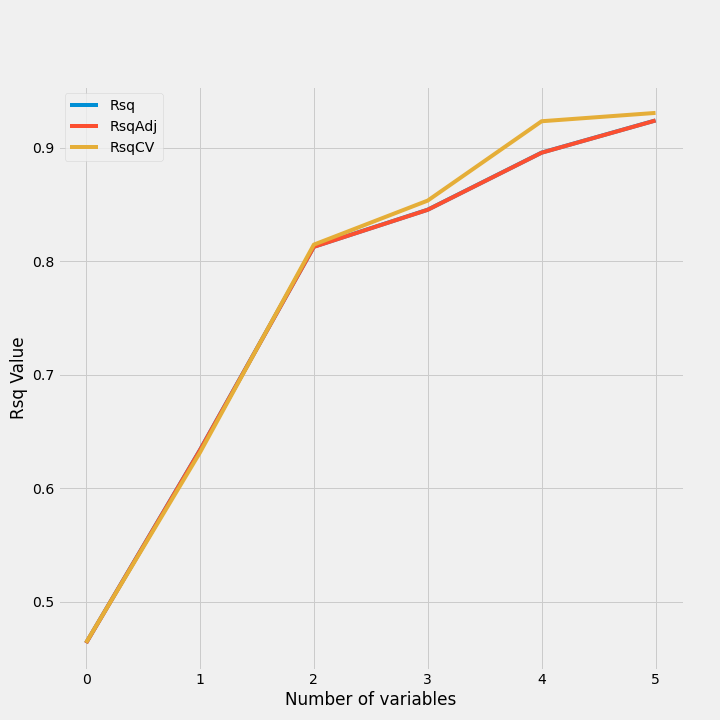
\includegraphics[scale = 0.2]{../plots/python/Stepwise3L.png}
	
	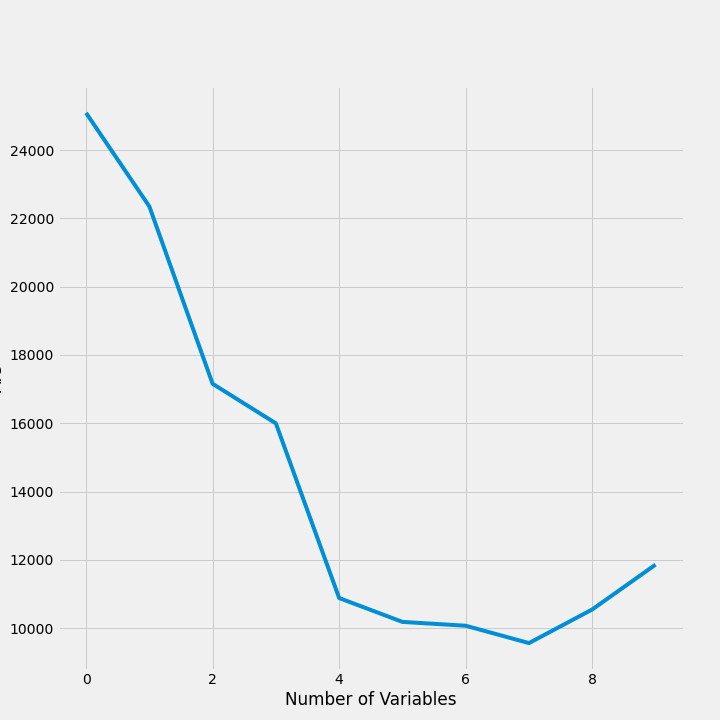
\includegraphics[scale = 0.2]{../plots/python/AICAutoForward3L.png} 
	\includegraphics[scale = 0.2]{../plots/python/AICBackward3L.png}
	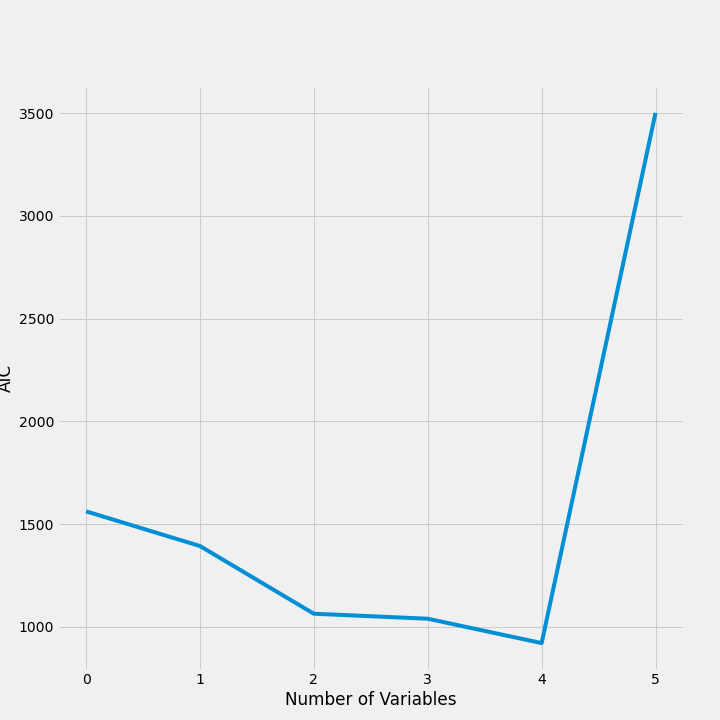
\includegraphics[scale = 0.2]{../plots/python/AICStepwise3L.png}
	
	4 Layer Network Selection Process (Forward, Backward, Stepwise)
	
	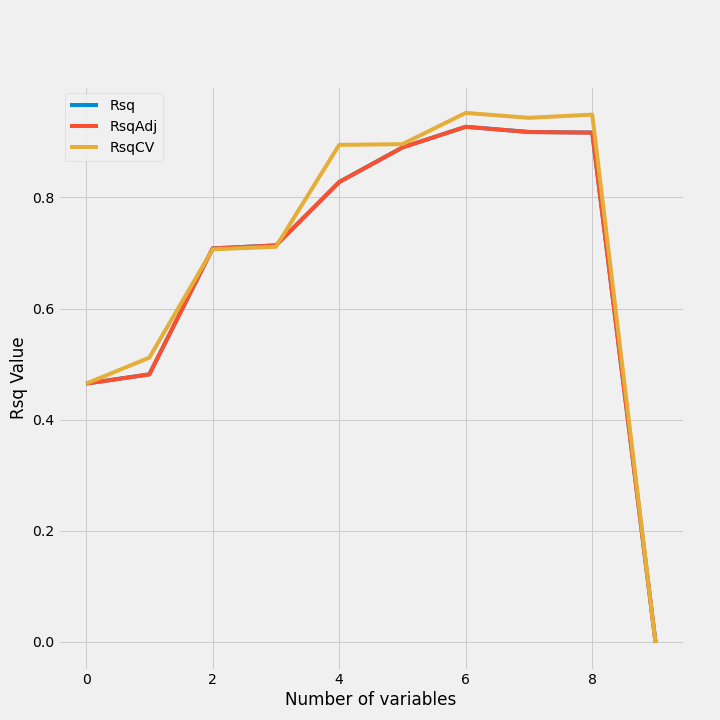
\includegraphics[scale = 0.2]{../plots/python/AutoForward4L.png} 
	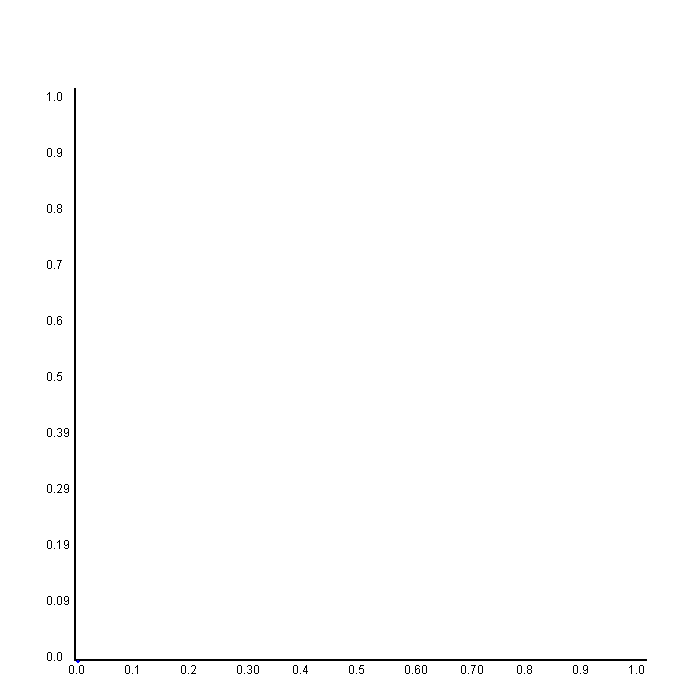
\includegraphics[scale = 0.2]{../plots/python/Backward4L.png}
	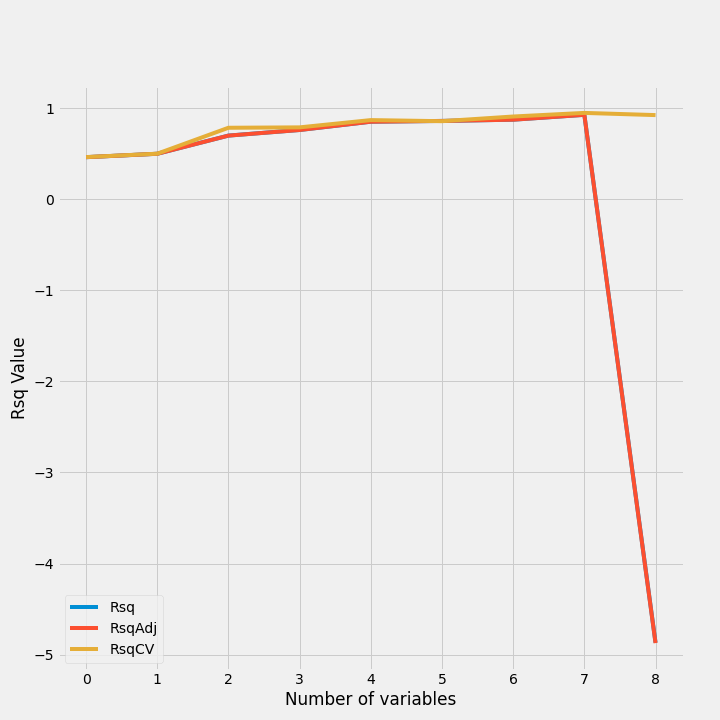
\includegraphics[scale = 0.2]{../plots/python/Stepwise4L.png}
	
	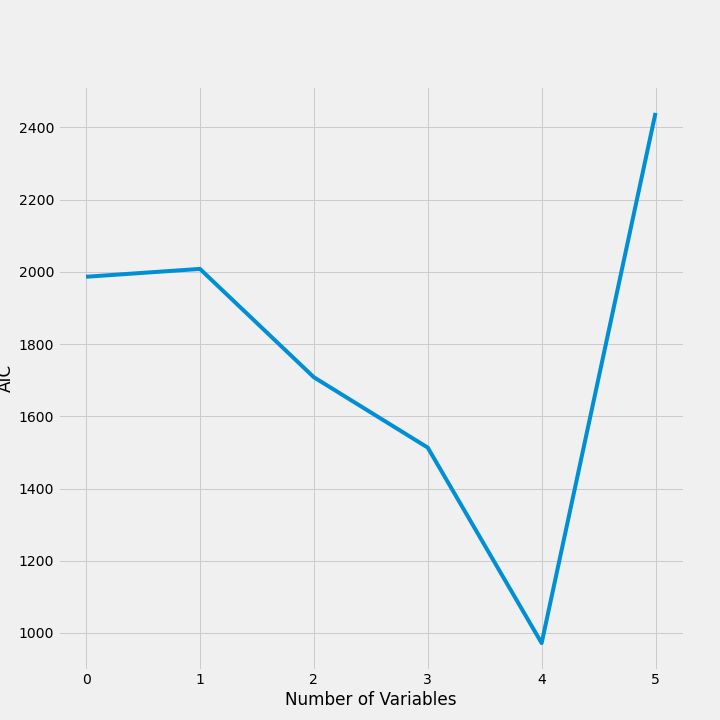
\includegraphics[scale = 0.2]{../plots/python/AICAutoForward4L.png} 
	\includegraphics[scale = 0.2]{../plots/python/AICBackward4L.png}
	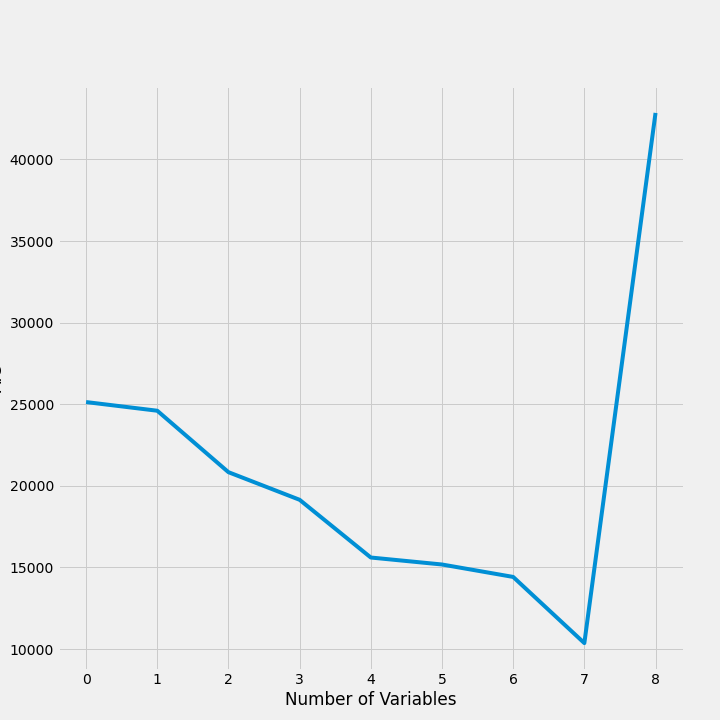
\includegraphics[scale = 0.2]{../plots/python/AICStepwise4L.png}
	
	As can be seen here is some very peculiar behavior with the model 
	occasionally failing to converge.
	
	\section{Concrete}
	
	The concrete compressive strength is a highly nonlinear function of age and ingredients used to determine the quality 
	of concrete. These ingredients include cement, blast furnace slag, fly ash, water, superplasticizer, coarse aggregate, 
	and fine aggregate. The Concrete Compressive Strength Data Set has 1,030 observations with a total of 9 attributes - 8 
	quantitative input variables, and 1 quantitative output variable. The data file can be found in the the data/ConcreteCompressiveStrength 
	folder, and were orignally downloaded from the UCI Machine Learning The dataset has the following variables: 
	
	\begin{enumerate}
		\item Cement (kg in a m3 mixture)
		\item Blast Furnace Slag (kg in a m3 mixture)
		\item Fly Ash (kg in a m3 mixture)
		\item Water (kg in a m3 mixture)
		\item Superplasticizer (kg in a m3 mixture)
		\item Coarse Aggregate (kg in a m3 mixture)
		\item Fine Aggregate (kg in a m3 mixture)
		\item Age (Day 1$\sim$365)
		\item Concrete (MPa) - the response variable
	\end{enumerate}

	\subsection{Results}

	Feed-forward neural networks will provide an advantage over 
	traditional regression modeling. Neural networks 
	are computationally expensive and require much more hyper parameter tuning than a traditional or 
	transformed regression model. The following table summarizes the results of our findings in terms 
	of $R^2$, $\bar R^2$ $R^2_{cv}$ and $AIC$ for some traditional regression models, and various neural networks. 
	

	\begin{tabular}{|c|c|c|}
		\hline
		& $R^2$ & $\bar R^2$ \\ \hline
		Multiple Linear Regression            & 0.614 & 0.612      \\ \hline
		Quadratic Regression                  & 0.768 & 0.766      \\ \hline
		Quadratic Regression with Cross Terms & 0.784 & 0.780      \\ \hline
		Transformed Regression                & 0.798 & 0.796      \\ \hline
		Perceptron                            & 0.654 & 0.632     \\ \hline
		3 Layer Neural Network                & 0.673 & 0.675      \\ \hline
		4 Layer Neural Network                & 0.642 & 0.648     \\ \hline
	\end{tabular}

	As the directly comparable results show (some results were not stable between python and scala) we can see that the neural 
	network models offer little to no benefit in comparison to the traditional regression models.
	
	\subsection{Variable Selection}
	
	Forward Selection, Backward Elimination, and Stepwise Regression for the 4 models. Below are graphs of the results.
	
	Perceptron Selection Process (Forward, Backward, Stepwise)
	
	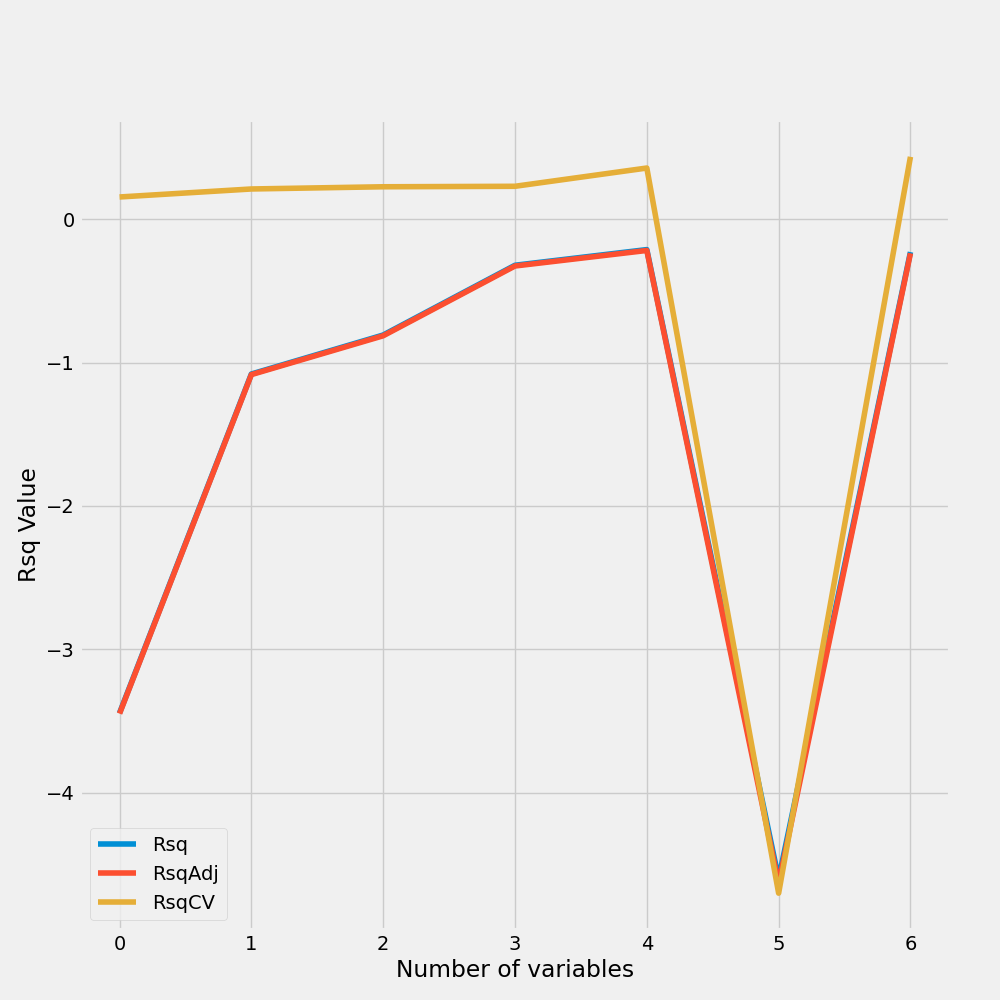
\includegraphics[scale = 0.2]{../plots/python/ConcreteForwardPCP.png} 
	\includegraphics[scale = 0.2]{../plots/python/ConcreteBackwardPCP.png}
	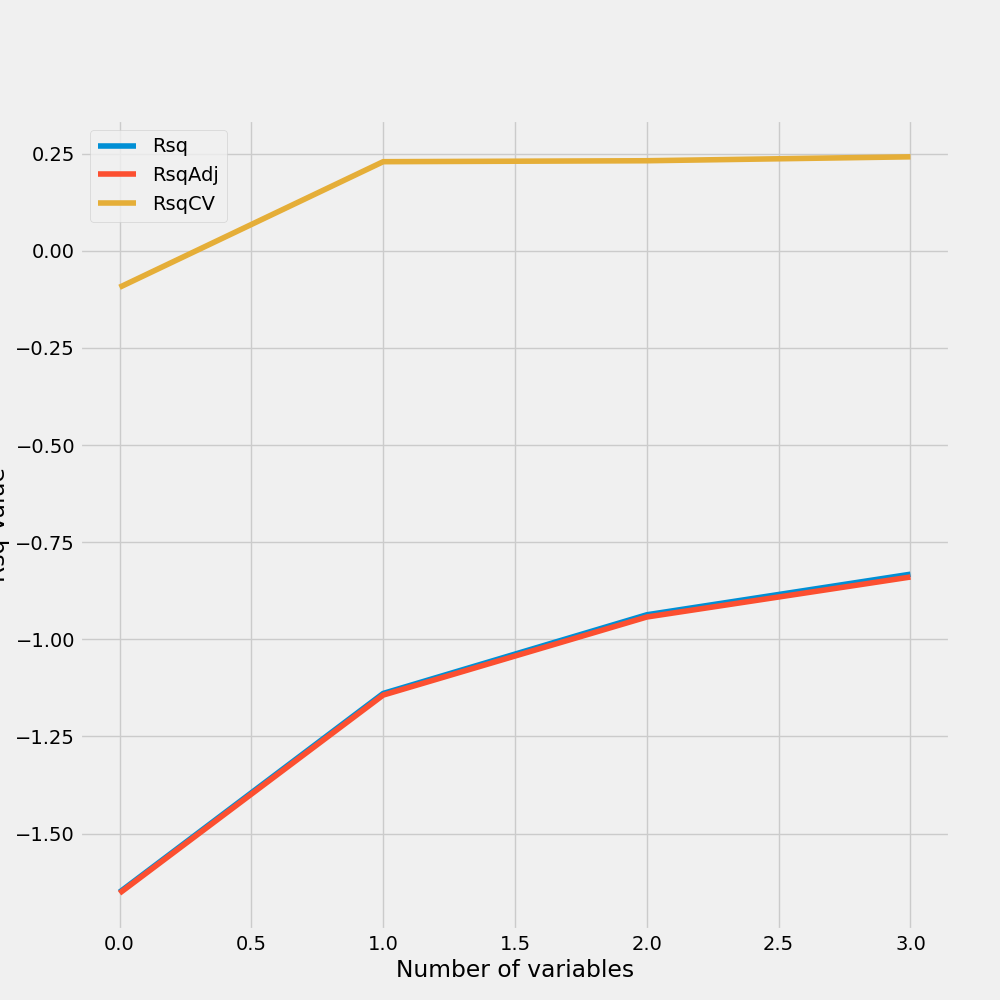
\includegraphics[scale = 0.2]{../plots/python/ConcreteStepwisePCP.png}
	
	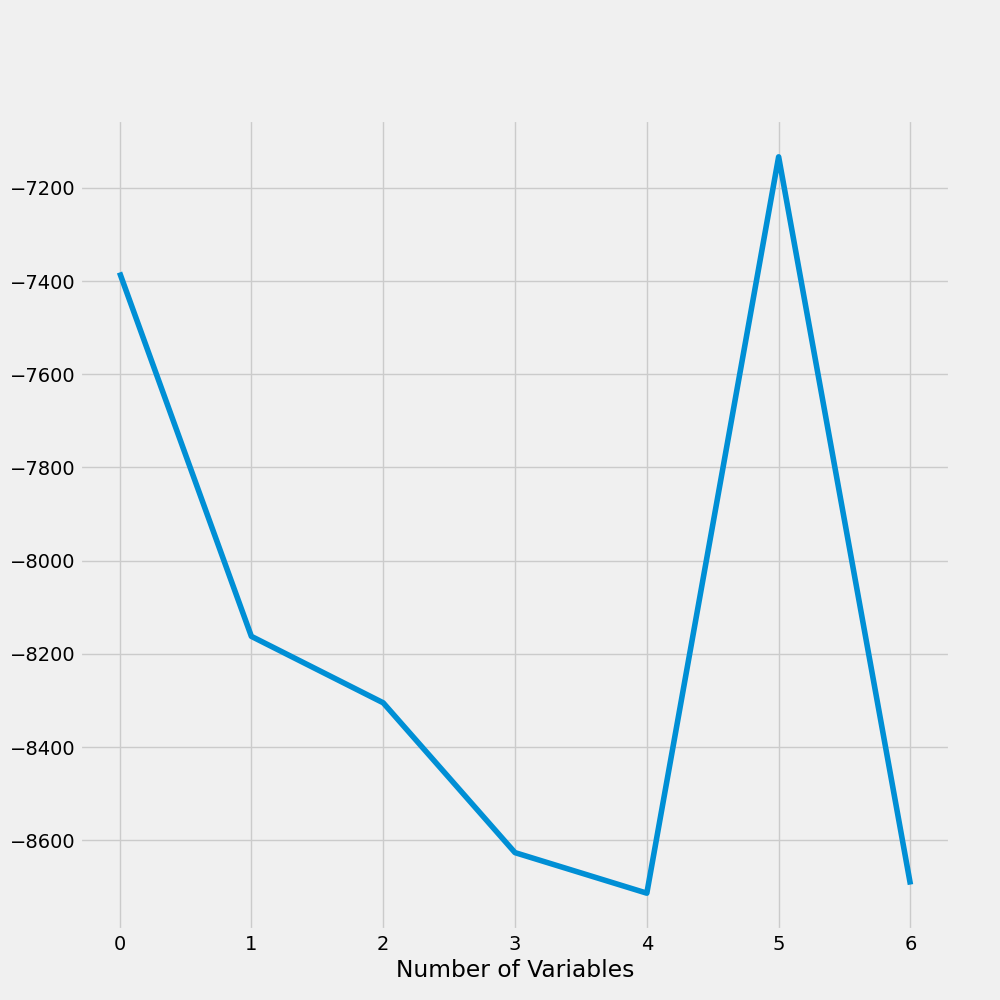
\includegraphics[scale = 0.2]{../plots/python/AICConcreteForwardPCP.png} 
	\includegraphics[scale = 0.2]{../plots/python/AICConcreteBackwardPCP.png}
	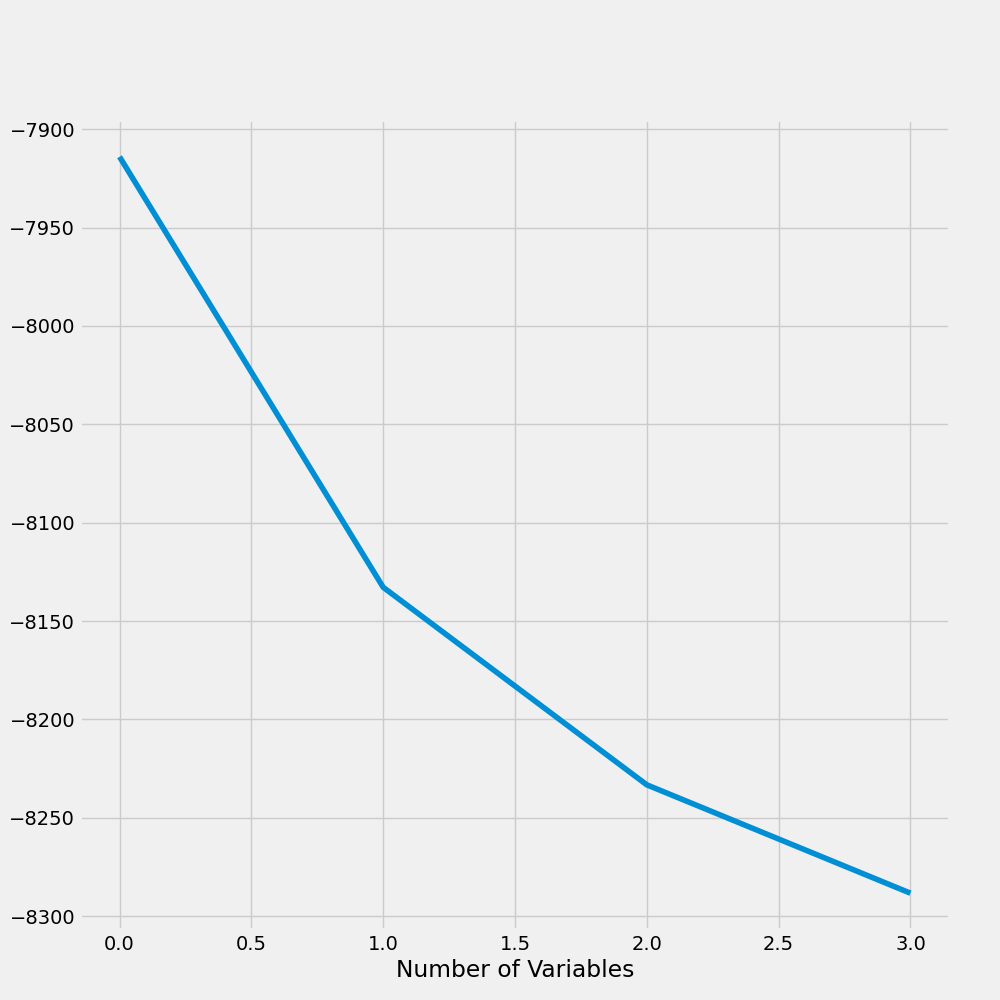
\includegraphics[scale = 0.2]{../plots/python/AICConcreteStepwisePCP.png}
	
	3 Layer Network Selection Process (Forward, Backward, Stepwise)
	
	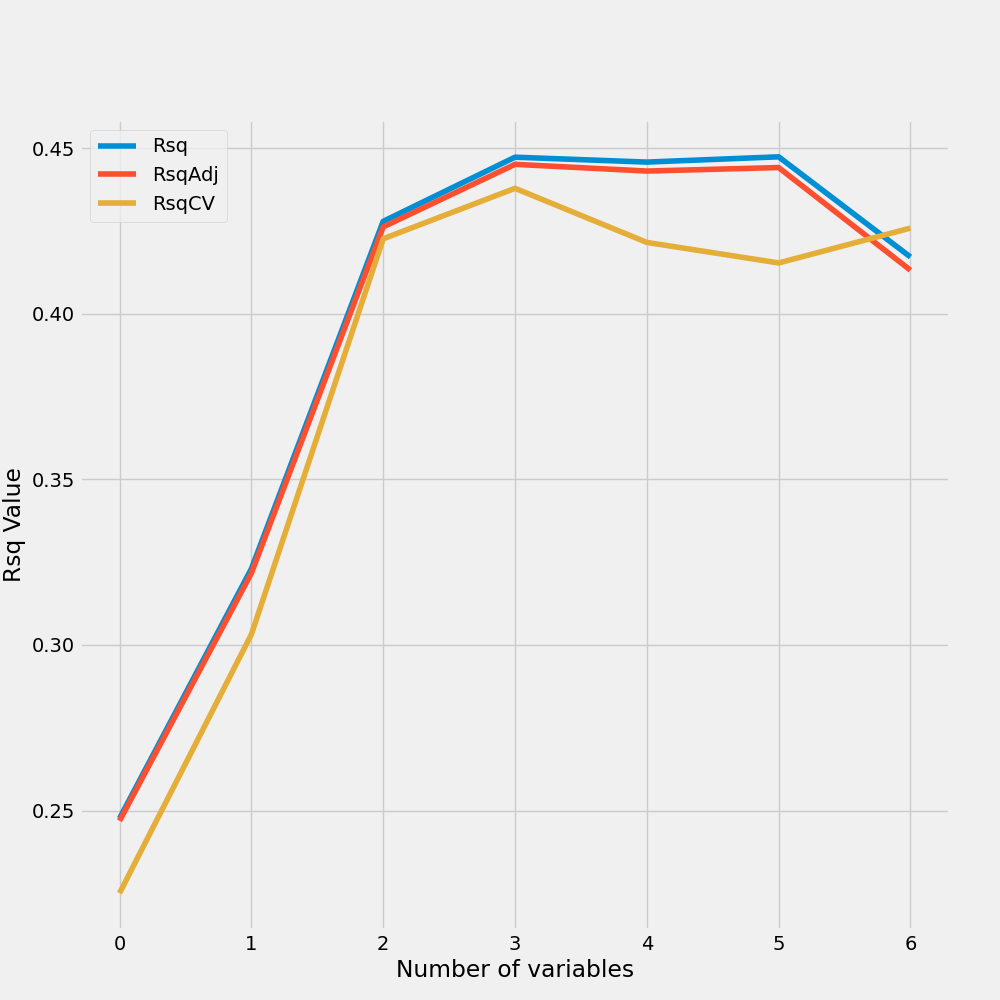
\includegraphics[scale = 0.2]{../plots/python/ConcreteForward3L.png} 
	\includegraphics[scale = 0.2]{../plots/python/ConcreteBackward3L.png}
	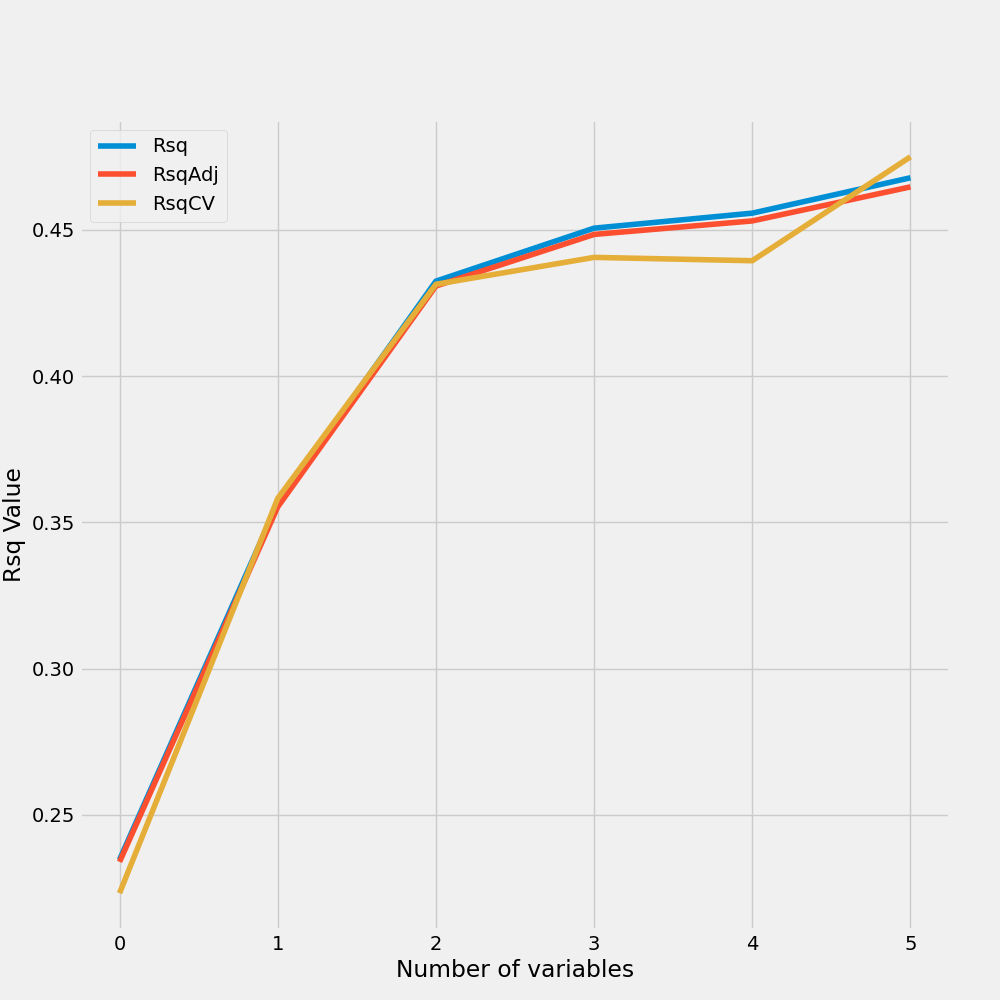
\includegraphics[scale = 0.2]{../plots/python/ConcreteStepwise3L.png}
	
	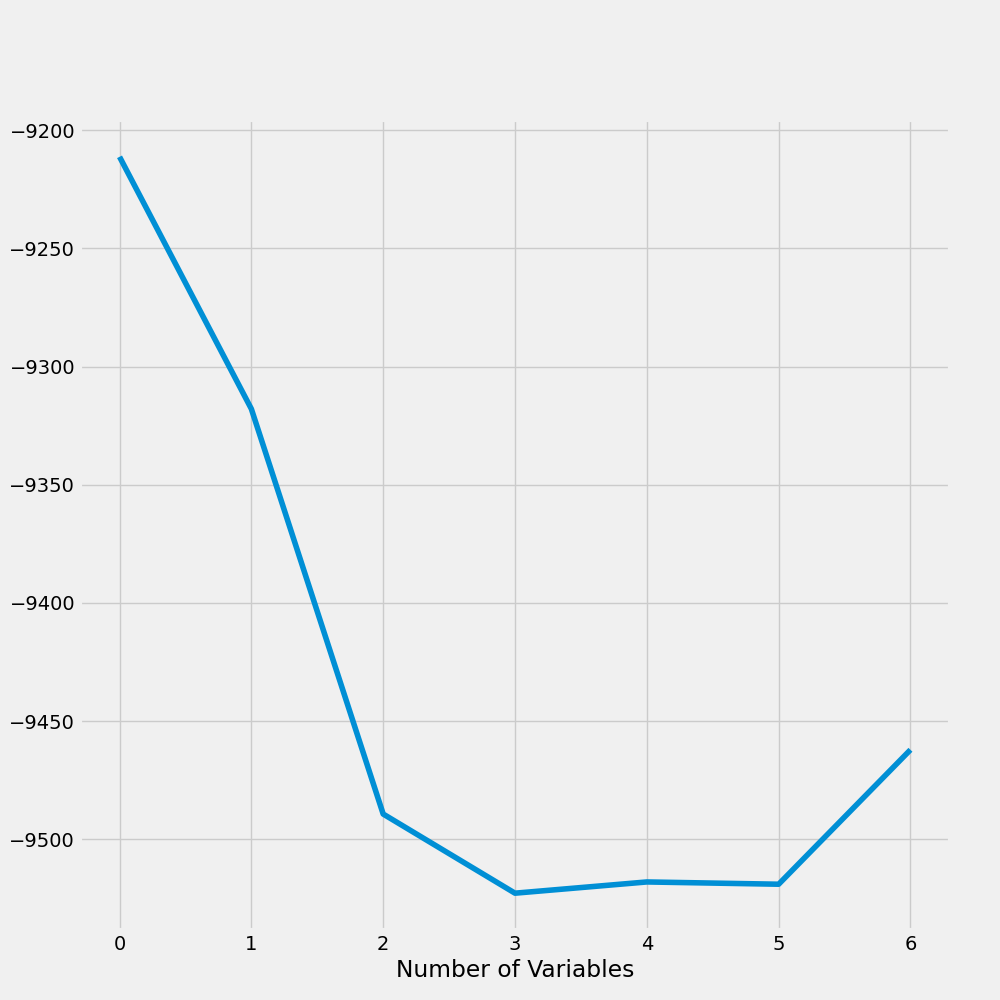
\includegraphics[scale = 0.2]{../plots/python/AICConcreteForward3L.png} 
	\includegraphics[scale = 0.2]{../plots/python/AICConcreteBackward3L.png}
	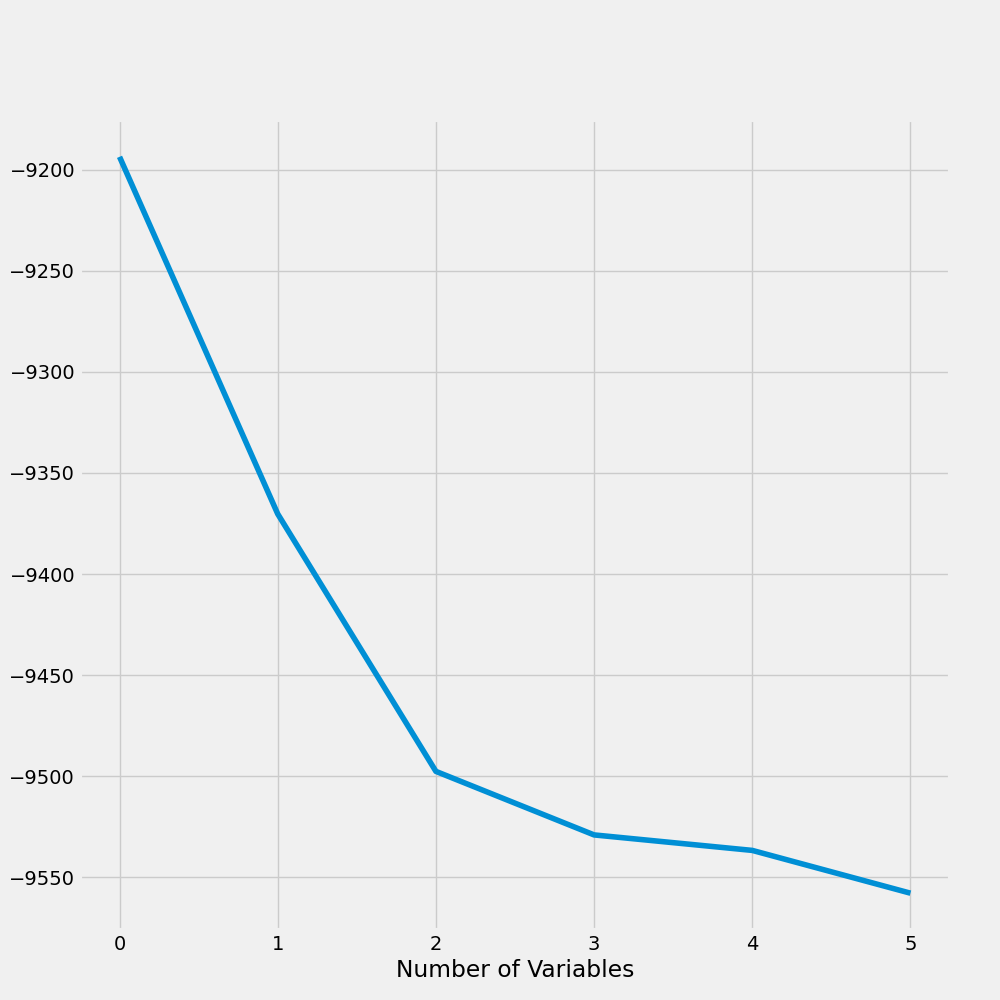
\includegraphics[scale = 0.2]{../plots/python/AICConcreteStepwise3L.png}
	
	4 Layer Network Selection Process (Forward, Backward, Stepwise)
	
	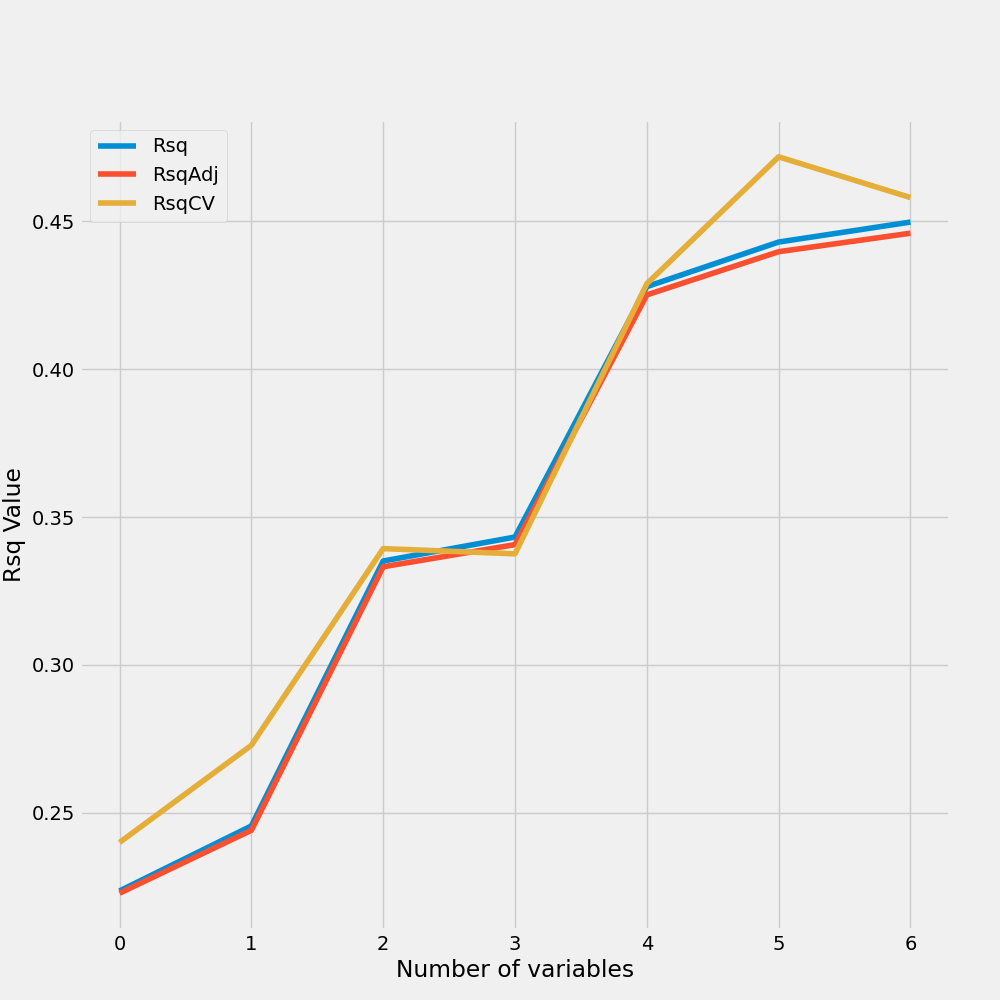
\includegraphics[scale = 0.2]{../plots/python/ConcreteForward4L.png} 
	\includegraphics[scale = 0.2]{../plots/python/ConcreteBackward4L.png}
	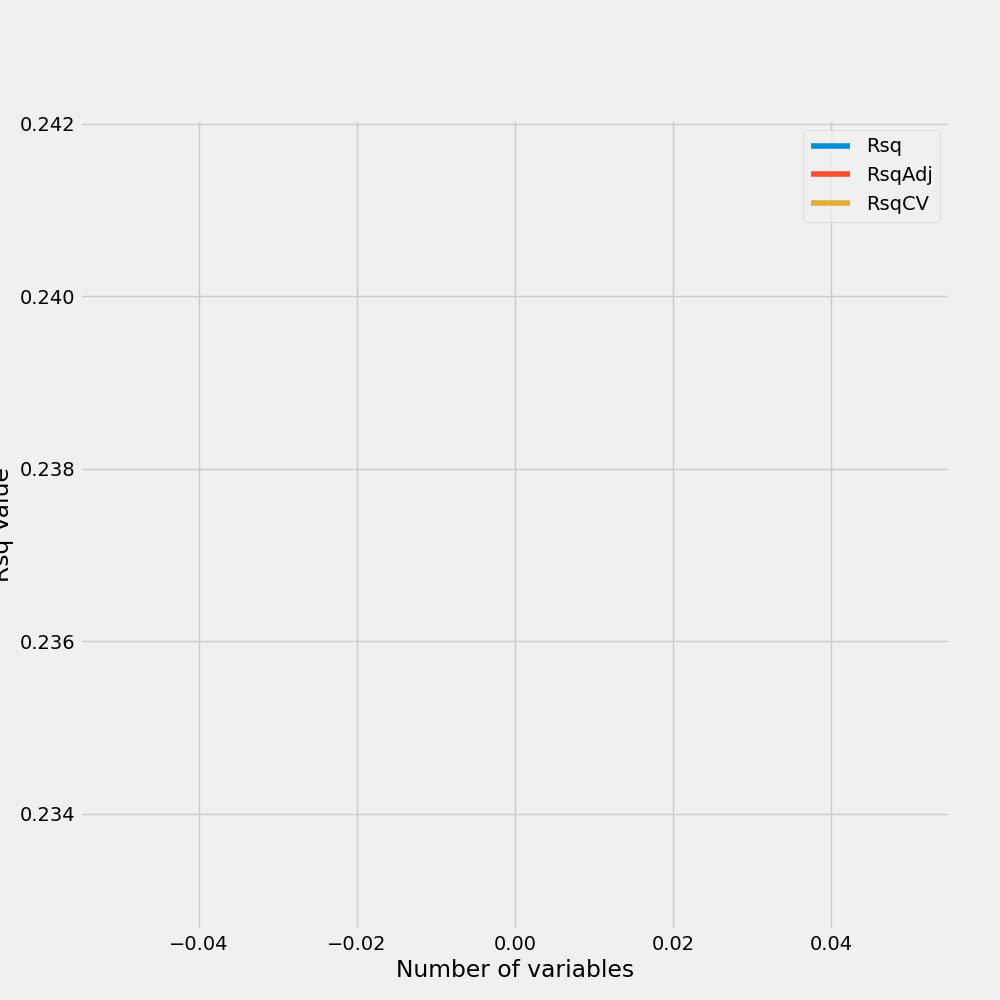
\includegraphics[scale = 0.2]{../plots/python/ConcreteStepwise4L.png}
	
	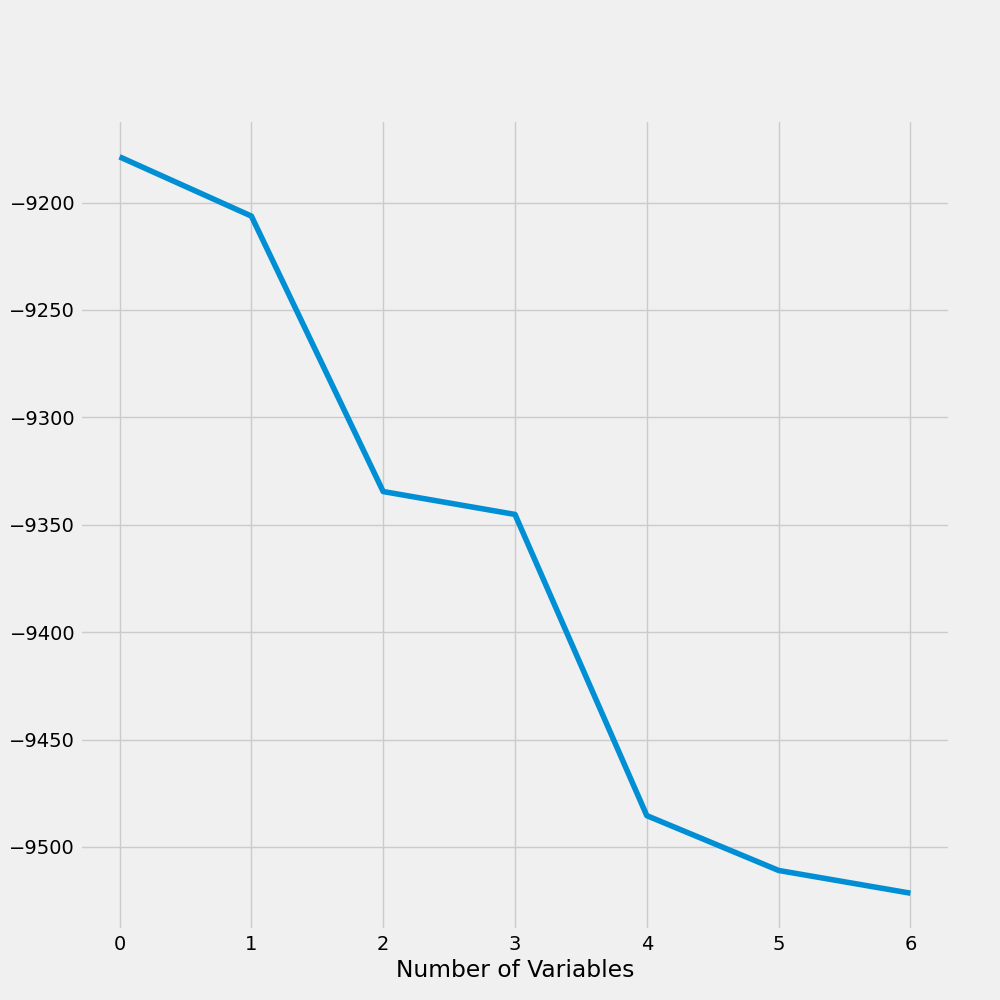
\includegraphics[scale = 0.2]{../plots/python/AICConcreteForward4L.png} 
	\includegraphics[scale = 0.2]{../plots/python/AICConcreteBackward4L.png}
	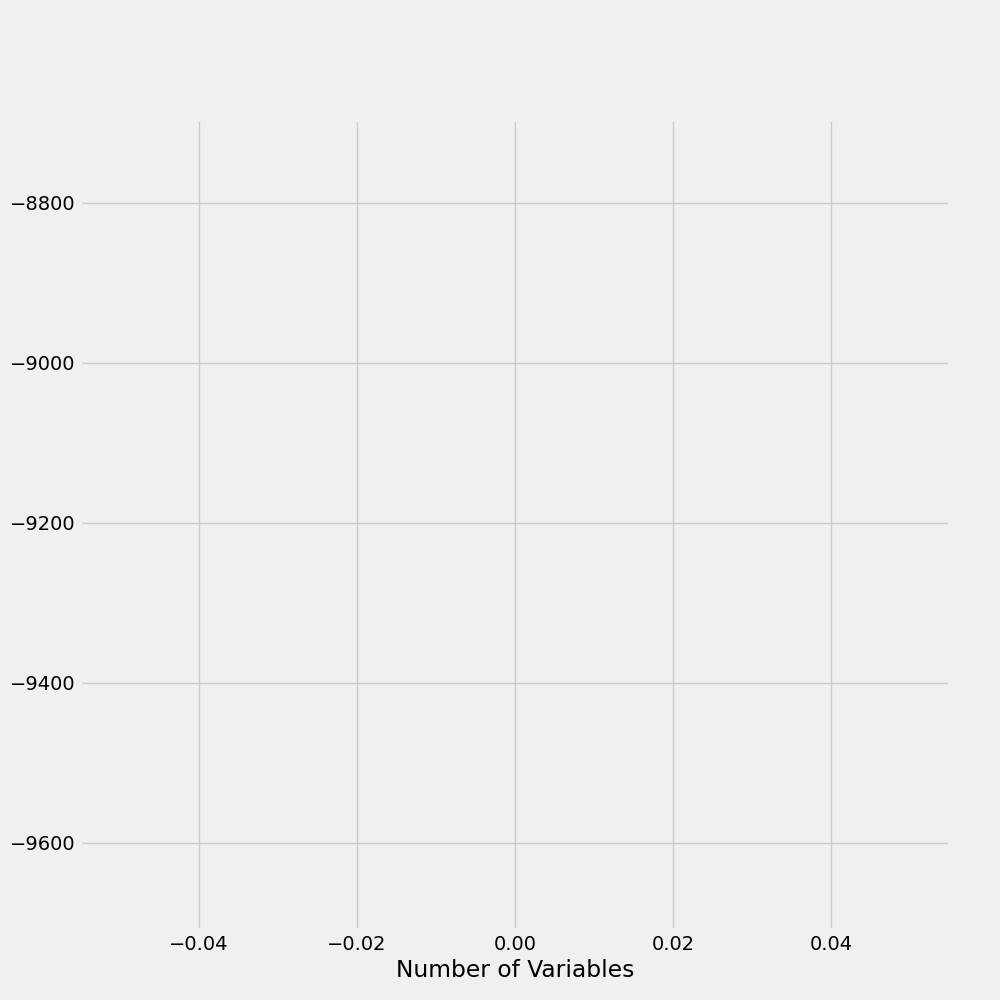
\includegraphics[scale = 0.2]{../plots/python/AICConcreteStepwise4L.png}
	
	As can be seen here is some very peculiar behavior with the model 
	occasionally failing to converge. 
	
	\section{Wine}
	
	The wine quality data is actually two datasets, one for red wine and the other for white 
	wine. Both of them have the same 11 features, but there may be differences in the features 
	that matter, as well as the overall results of regression. A dummy variable could be created 
	to meld the datasets into one overall set, but if there are substantial differences between 
	the two it may substantially add to model complexity. The dataset has the following variables: 
	
	\begin{enumerate}
		\item fixed.acidity 
		\item volatile.acidity 
		\item citric.acid 
		\item residual.sugar 
		\item chlorides 
		\item free.sulfur.dioxide 
		\item total.sulfur.dioxide 
		\item density
		\item pH
		\item sulfates 
		\item alcohol 
		\item quality (the response variable)
	\end{enumerate}

	The red wine dataset has 1,599 observations, and the white wine dataset has 4,898 observations. 
	The two files can be found in the data/WineQuality folder, and were orignally downloaded from 
	the \href{https://archive.ics.uci.edu/ml/datasets/wine+quality}{UCI Machine Learning Repository}. 

	\subsection{Results}

	Feed-forward neural networks will provide an advantage over 
	traditional regression modeling. Neural networks 
	are computationally expensive and require much more hyper parameter tuning than a traditional or 
	transformed regression model. The following table summarizes the results of our findings in terms 
	of $R^2$, $\bar R^2$ $R^2_{cv}$ and $AIC$ for some traditional regression models, and various neural networks. 
	

	\begin{tabular}{|c|c|c|}
		\hline
		& $R^2$ & $\bar R^2$ \\ \hline
		Multiple Linear Regression            & 0.614 & 0.612      \\ \hline
		Quadratic Regression                  & 0.768 & 0.766      \\ \hline
		Quadratic Regression with Cross Terms & 0.784 & 0.780      \\ \hline
		Transformed Regression                & 0.798 & 0.796      \\ \hline
		Perceptron                            & 0.654 & 0.632     \\ \hline
		3 Layer Neural Network                & 0.673 & 0.675      \\ \hline
		4 Layer Neural Network                & 0.642 & 0.648     \\ \hline
	\end{tabular}

	As the directly comparable results show (some results were not stable between python and scala) we can see that the neural 
	network models offer little to no benefit in comparison to the traditional regression models.
	
	\subsection{Variable Selection}
	
	Forward Selection, Backward Elimination, and Stepwise Regression for the 4 models. Below are graphs of the results.
	
	Perceptron Selection Process (Forward, Backward, Stepwise)
	
	\includegraphics[scale = 0.2]{../plots/python/WineForwardPCP.png} 
	\includegraphics[scale = 0.2]{../plots/python/WineBackwardPCP.png}
	\includegraphics[scale = 0.2]{../plots/python/WineStepwisePCP.png}
	
	\includegraphics[scale = 0.2]{../plots/python/AICWineForwardPCP.png} 
	\includegraphics[scale = 0.2]{../plots/python/AICWineBackwardPCP.png}
	\includegraphics[scale = 0.2]{../plots/python/AICWineStepwisePCP.png}
	
	3 Layer Network Selection Process (Forward, Backward, Stepwise)
	
	\includegraphics[scale = 0.2]{../plots/python/WineForward3L.png} 
	\includegraphics[scale = 0.2]{../plots/python/WineBackward3L.png}
	\includegraphics[scale = 0.2]{../plots/python/WineStepwise3L.png}
	
	\includegraphics[scale = 0.2]{../plots/python/AICWineAutoForward3L.png} 
	\includegraphics[scale = 0.2]{../plots/python/AICWineBackward3L.png}
	\includegraphics[scale = 0.2]{../plots/python/AICWineStepwise3L.png}
	
	4 Layer Network Selection Process (Forward, Backward, Stepwise)
	
	\includegraphics[scale = 0.2]{../plots/python/WineForward4L.png} 
	\includegraphics[scale = 0.2]{../plots/python/WineBackward4L.png}
	\includegraphics[scale = 0.2]{../plots/python/WineStepwise4L.png}
	
	\includegraphics[scale = 0.2]{../plots/python/AICWineForward4L.png} 
	\includegraphics[scale = 0.2]{../plots/python/AICWineBackward4L.png}
	\includegraphics[scale = 0.2]{../plots/python/AICWineStepwise4L.png}
	
	
\end{document}
